\documentclass[titlepage]{article}
\usepackage[
  sorting=none,
  citestyle=ieee,
  style=ieee]{biblatex}
\addbibresource{bibliography.bib}
\usepackage{fancyhdr}
\usepackage{enumitem}
\setlist[enumerate]{label*=\arabic*.} 
\usepackage{graphicx}
\graphicspath{ {./images/} }

\pagestyle{fancy}
\fancyhf{}
\rhead{COMP2043.GRP Interim Group Report}
\lhead{Team02}

\begin{document}

\begin{titlepage}
  \centering
  \large{\textsc{COMP2043.GRP Interim Group Report}}\\
  \vspace{3cm}
  \huge{Team02}\\
  \Huge{Machine Learning Dataset Parsing Tool}\\
  \vspace{3cm}
  \LARGE{\textsc{Group Members}}\\
  \Large{Boyuan Ma - zy22053 (Team Leader)}\\
  \Large{Xinyan Li - zy22043}\\
  \Large{Hao Liu - zy22046}\\
  \Large{Xinjie Pang - zy22055}\\
  \Large{Marios Igkiempor - scymi1}\\
  \vspace{1cm}
  \LARGE{\textsc{Supervisor}}\\
  \Large{Chris Roadknight}\\
  \vfill
  \large{\textsc{December 2018}}
  
\end{titlepage}

\tableofcontents
\pagebreak

\section{Description of the Problem}
Team02's project is centered around a system that classifies datasets by the best type of machine learning approach to take in order to best analyse the data. It is proposed that the system will be able to parse a dataset, analyse its features and propose a type of machine learning (supervised, semi-supervised and unsupervised), as well as a more specific algorithm, that can best model the dataset based on the analysed features.

The client intends to use the project as both a prefilter for machine learning and as a teaching aid, and so the program should be able to provide useful information as to how the machine learning approach was derived. However, it should be noted that being an expert in the field, the client expects his knowledge to be captured in the system. As such, any useful information provided by the system would be used to aid the teaching of students and should therefore be suitable for someone that is not an expert in the field.

Datasets that the program will analyse will be provided by the client, however the system should be able to parse and analyse newly uploaded datasets with the same level of accuracy.

\section{Background Information and \\Relevant Research}
\subsection{Machine Learning}
The team has to figure out how many machine learning methods would be provided in our website, their respective principles, and how and when to use each one.
There exist many open source machine learning toolkits such as H2o \cite{h2o.ai}, Weka \cite{weka} and various Python and R packages. These machine learning toolkits could be used to analyze different datasets. In this early stage of the project, the team has chosen to use Weka to understand each machine learning method.

\subsection{Understanding Machine Learning Algorithms}
Section \ref{pickingML} lists the machine learning algorithms that the system will be able to produce as output. The team felt it would be beneficial to have a basic understanding of each algorithm and where it is most useful. Some background research was conducted into each algorithm.

\subsubsection*{Self-Organising Map (SOM)}
% A Self-Organising Map (SOM) is an unsupervised system is based on competitive learning, in which competition between the output neurons is activated, with the result that only one neuron is activated at any time. This activated neuron is called the winner neuron (the winner is king-all neuron). This competition can be achieved by having a laterally suppressed connection (negative feedback path) between the neurons. The result is that neurons are forced to recombine themselves, such a network we call self-organizing maps (SOM).
\subsubsection*{K-Means Clustering}
% K-means clustering is an algorithm that classifies data into $k$ groups based on the characteristics of the data. $k$ is a positive integer. The grouping is assigned to the corresponding group based on the smallest square of the distance between the original data and the cluster centroid.
K-means clustering classifies a set of data into $k$ clusters (where $k > 0$) by assigning it to a centroid (central location of a cluster). This is achieved by assigning it to the nearest centroid. When each data point has been assigned, $k$ centroids are recalculated and the datapoints are reassigned. This process of defining and assigning to new centroids is repeated until no data points move.\cite{kmeans}
\subsubsection*{Principal Component Analysis}
% Principal Component Analysis (PCA) transforms the original data into a set of linearly independent representations of each dimension through linear transformation, which can be used to extract the main feature components of the data, which is often used for dimensionality reduction of high-dimensional data.
\subsubsection*{Linear Regression}
% Linear regression is a statistical analysis method that uses the regression analysis in mathematical statistics to determine the quantitative relationship between two or more variables. Its expression is $y = w'x+e$, where $e$ is a normal distribution with an error obeying a mean of $0$.
\subsubsection*{Neural Network}
Artificial Neural Network (ANN) is a machine learning method simulating information processing of a human brain to build a mathematic model. The model consists of processing elements (neurons) which each have an activation function. ANNs require a large amount of examples as training data and test data to complete the model, like the process of human learning. It has advantages in processing amounts of fuzzy nonlinear data.
\subsubsection*{Multiclass Neural Network}
% Firstly, using Logistic Regression to do Multi-Category classification. With one-to-many logistic regression, in order to make training more efficient, it needs to be vectorized to avoid loop operations. For each input data, there is a 1*10 vector, which corresponds to a probability of 0~9. Then add a Hidden layer between the input and output layer, which is Multiclass Neural Network.
\subsubsection*{Random Forest Regression}
% It performs many times of sampling back to the original data set, and each time extracts the same number of observations as the sample size. Since it is put back into the sample, some observations are not drawn each time, and some observations are repeatedly drawn. You get a lot of different data sets and then build a decision tree for each data set, thus generating a large number of decision trees.
\subsubsection*{Logistic Regression}
Logistic Regression is a method for binary prediction when the outputs are dichotomous (true or false). The weight of independent variables can be deduced by Logistic Regression when the binary outputs (dependent variable) are provided. The probability of output can also be predicted by the regression model. It is generally used for data mining, disease analysis and economic projection.
\subsubsection*{Multiclass Logistic Regression}
% Firstly, using Logistic Regression to do Multi-Category classification. With one-to-many logistic regression, in order to make training more efficient, it needs to be vectorized to avoid loop operations. For each input data, there is a 1*10 vector, which corresponds to a probability of 0~9. Then add a Hidden layer between the input and output layer, which is Multiclass Neural Network.
\subsubsection*{Naïve Bayesian Network}
Naïve Bayes is a sorting technique based on Bayes’ theorem. It sets characteristics of data as tags and assume that the tags are mutually independent on probability. Then the Naïve Bayes Classifier sort the objects and calculates probability according to these tags. And the objects can be sorted to known classes or demonstrate the probability of an object belonging to a class.
\subsubsection*{Support Vector Machine}
Support Vector Machine (SVM) is a method used to sort and regress. SVM is a development of binary liner classifier. For the nonlinearities, SVM transforms the sample into higher dimensions so that the sample can be linerly analyzed because of high dimensional features.
\subsubsection*{Self-Training}
Self-Training is a semi-supervised learning method. It divides first divides sample data into labelled and non-labelled subcategories. Because of high accuracy of classifier, the model can be used to label the unlabeled data sets. Then the unlabeled data can be deleted. The Algorithm will repeat these steps until the datasets not change any more.
\subsubsection*{Forced Clustering}
\subsubsection*{Anti-Learning}
Anti-learning is used when the accuracy of a trained model's output is worse than random outputs even if no overfitting or over training occurred.

\section{Requirements Specification}
Following meeting with the client and discussing initial user requirements and system requirements specification, as well as subsequent meeting revising both requirements, the team and the client have agreed on a set of requirements.

\subsection{User Requirements}

\begin{enumerate}
  \item Parse datasets and suggests the best machine learning approaches for modeling that dataset.

  \item The user will supply datasets to be analysed.
  
  \item The system will need to be appropriate for use as both a prefilter for machine learning and as a teaching aid.
  
  \item The user requires a degree of data visualization in the front end.
  
  \item The user requires a comprehensive, extendible database. The database should allow the user to:
  \begin{enumerate}
    \item upload datasets
    \item provide relevant information about the datasets
  \end{enumerate}
  
  \item A rule-based approach will initially be sufficient to assertain what the ideal machine learning approach is for each dataset. The user should be able to affect the decisions made by the rule based system by providing additional information on the structure and complexity of the data.
  
  \item The client has significant knowledge of machine learning methods and some of this knowledge will be captured to facilitate the decision making process.
\end{enumerate}

\subsection{Functional System Requirements}

\begin{enumerate}
  \item The system will require a database which can store the data in every dataset
  
  \begin{enumerate}
    \item The user can upload the dataset.
  
    \item The datasets are available for users to download.
    
    \item Information about the dataset (what type of data, whether or not there are missing values) can be provided by the user and stored as metadata with each dataset.
    
    \item The datasets need preprocessing to find details about the data. These details must be stored as metadata with the dataset. Details will be characteristics of the datasets which help decide the best machine learning approach. Such details could include:
    \begin{enumerate}
      \item The type of data
      \item Size of the dataset
      \item Number of features
      \item Number of target outputs provided with the data
      \item Whether or not there are missing values
      \item Whether the labels are categories or values
      \item Complexity of the dataset
      \item Complexity of relations in the dataset
      \item Wether or not the dataset is structured
    \end{enumerate}

    \item The customer needs to be able to add and delete information stored in the database.
    
    \item The original data must never be altered. Any pre-processing or analysis may be available to the user, but the user must also have access to the original data they provided.
  \end{enumerate}
  
  \item The system must be able to analyze a dataset and provide the best machine learning approach to model the dataset.
  \begin{enumerate}
    \item The reason why that approach is best needs to be provided to the user.
  
    \item The system will have different cataglogues of machine learning. Each cataglogue provides the algorithm for the machine learning and the sample datasets.
    
    \item The system must have a search engine which can search for both the datasets' name and machine learning approaches.
  \end{enumerate}
  
  \item The system must provide different types of data visualization
  \begin{enumerate}
    \item Bar charts
    \item Scatter graphs
    \item Images 
    \item Interactive visualization at the result page
  \end{enumerate}
  
  \item The system should have different mapping opinions for finding the ideal machine learning method:
  \begin{enumerate}
    \item Rule-based system
    \item Deterministic mode
    \item Probabilistic mode
  \end{enumerate} 

  \item As a long-term goal, the system could actually model the data using the decided machine learning tool and provide a visual output of the model for the user.
\end{enumerate}

\subsection{Non-Functional System Requirements}
\begin{enumerate}
  \item Accessibility
  \begin{enumerate}
    \item The user should be able to upload data using multiple types of input, for example both the mouse and the keyboard.
    \item The system should be accessible on multiple different platforms.
  \end{enumerate}

  \item Data integrity
  
  The original uploaded data should never be changed. If there are mechanisms in place which change the data, these should not affect the original data

 \item Data Retention
  
  Data stored on the sever should only be kept there for 30 days as a limit.

  \item Extensibility

  The system should be able to cope with data of no more than 200MB.

 \item Performance:

  The system should be able to analyse new data sets in no longer than 1 minute.

  \item Privacy and Security:

  Data uploaded by a user must have the option to be kept private to the user who uploaded it.
\end{enumerate}

\subsection{Modelling Requirements}
Following the elicitation of user and system requirements, the team decided it was useful to model both. A simple use case diagram was created first, shown in figure \ref{usecase}.

\begin{figure}[h!]
  \centering
  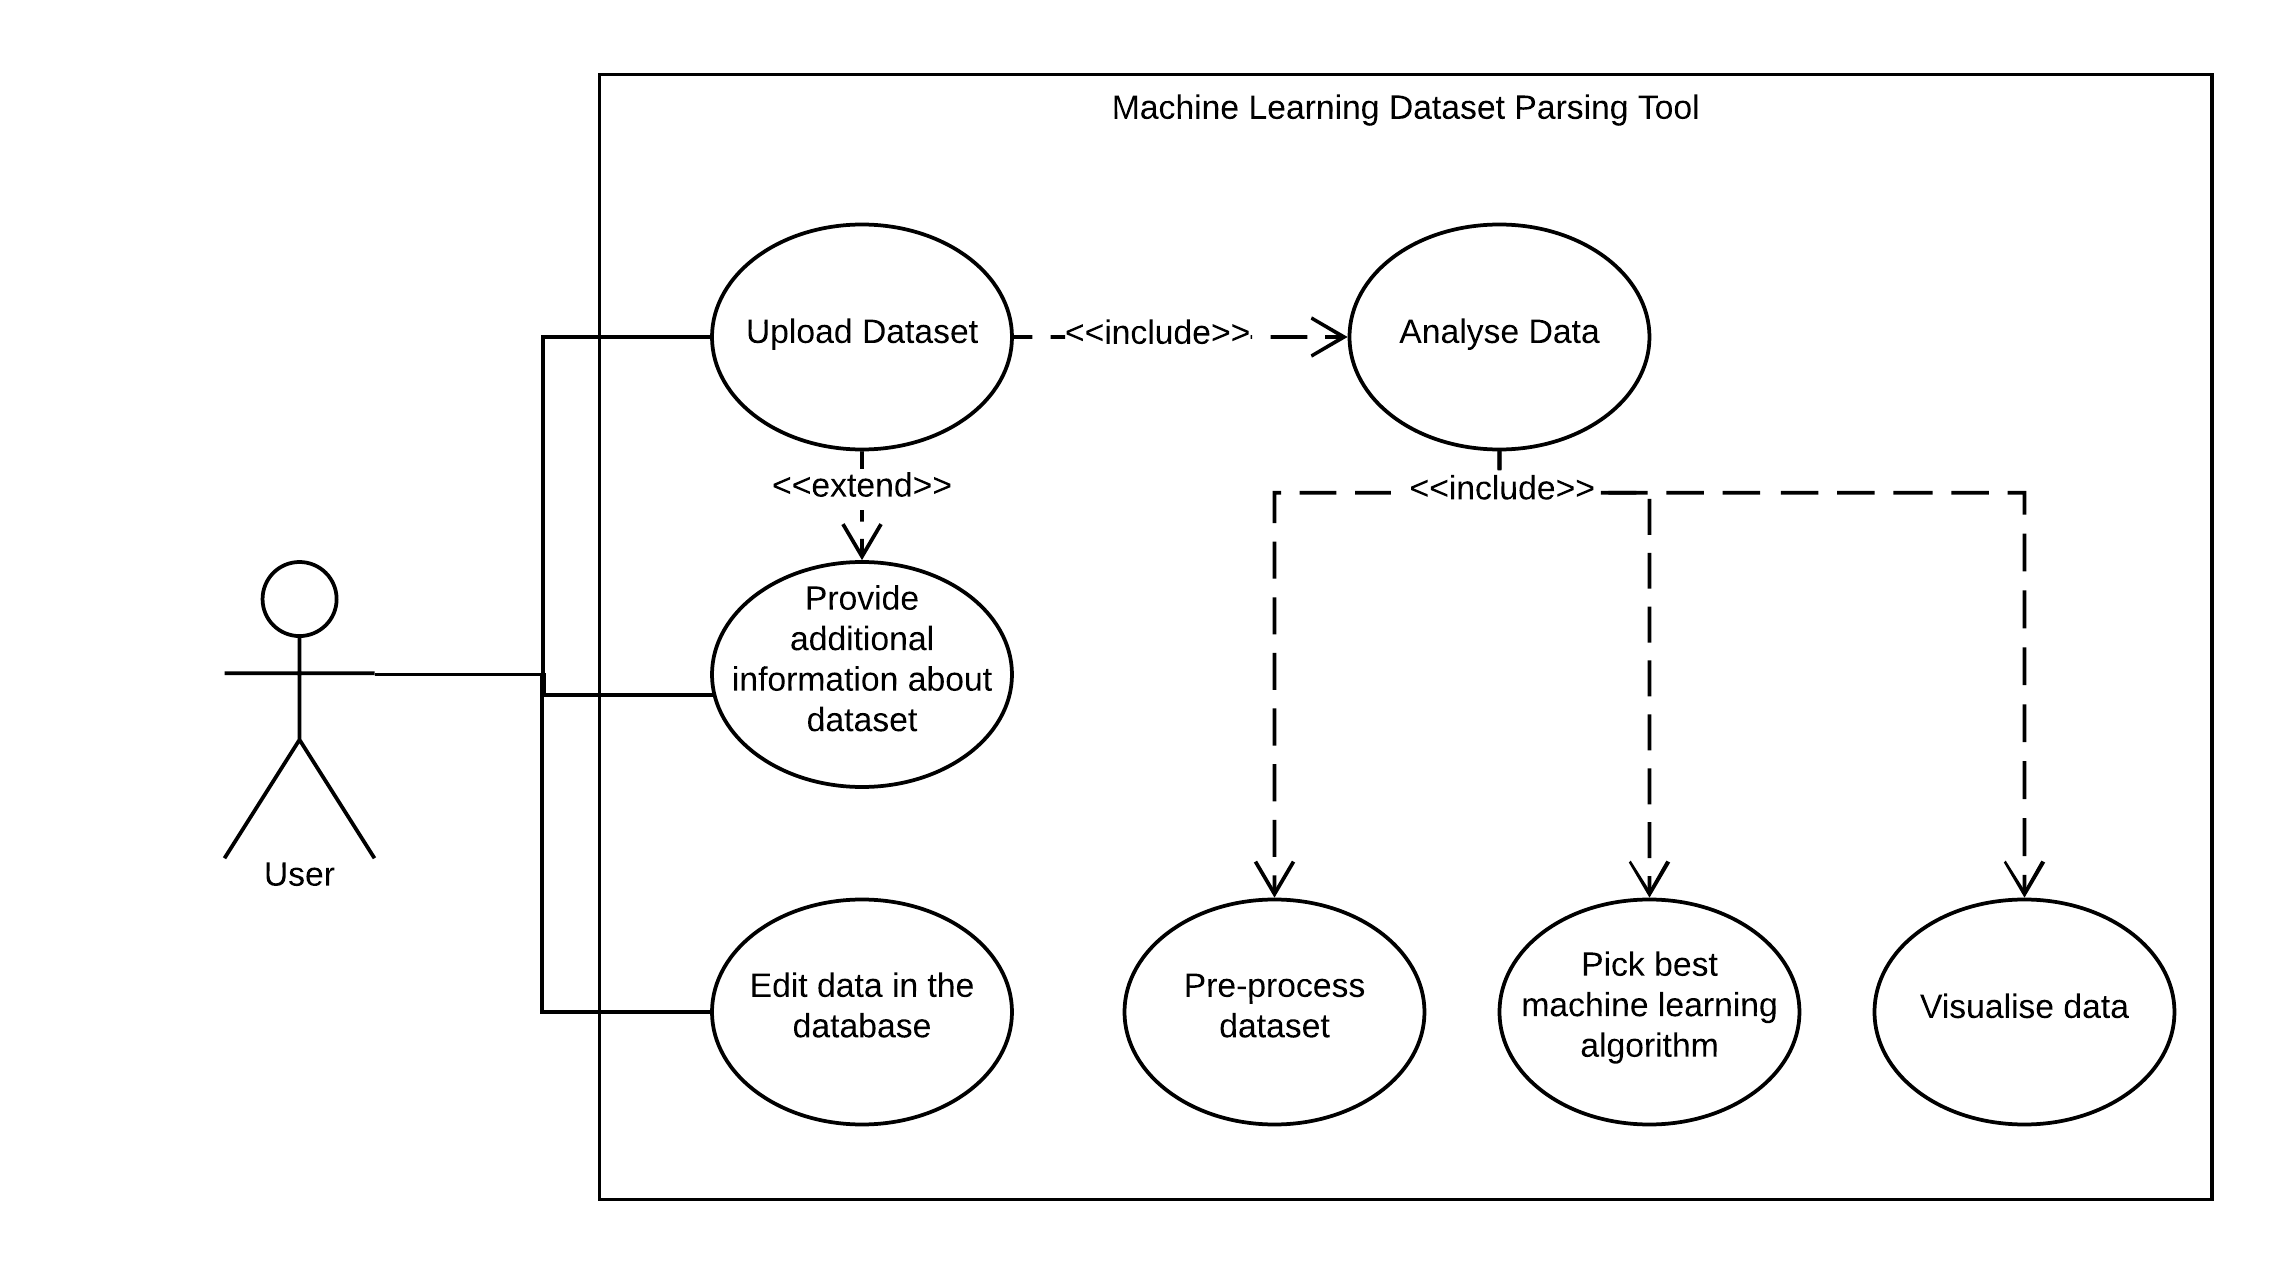
\includegraphics[width=\textwidth]{usecase}
  \caption{Simple use case diagram of the system}
  \label{usecase}
\end{figure}

The use case diagram clearly shows how the user will interact with the system. Due to the nature of the system, much of its complexity is hidden from the user and therefore the user does not have many use cases. Regardless, the use case diagram is an important part of the requirements gathering process as it makes it easier for the client to visualise their interactions with the system.

\section{Initial Design Ideas}
\subsection{Picking the Machine Learning Approach} \label{pickingML}
The final goal of the project is to analyze datasets and automatically suggest the best machine learning tools by using our machine learning analyzer. The analyzer will initially be composed of a Decision Tree, which will identify the best machine learning approach based on features of a given dataset.

The short-term goal is to classify dataset into three broad categories: Supervised Learning, Unsupervised Learning and Semi-supervised Learning according to whether there is output data in the dataset. In order to provide a prototype to the client, the system will pick a random machine learning approah. This will let the client have an idea of what a working system would function like.

The team decide to provide 17 potential machine learning tools:
\begin{itemize}
  \item Multiclass Neural Network
  \item Linear Regression
  \item Random Forest Regression
  \item Sum Regression
  \item Logistic Regression
  \item Neural Network
  \item NB or Sum
  \item Anti-learning
  \item Self-Organizing Map
  \item K-means Clustering
  \item Principle Component Analysis
  \item Forced Clustering
  \item Self-Training
  \item Deep Learning
  \item Recurrent Neural Network
  \item Time Delay Neural Network
  \item Feature Selection Principal Component Analysis
\end{itemize}
The most suitable tool will be suggested from this list of machine learning methods by using decision algorithm in the second iteration of the project, after the prototype.

The website will display the selected most suitable machine learning tool for each dataset uploaded by client. In the long term, the team hopes that the website will be able to analyze the dataset by using the best machine learning tool and visualize the output. However, the team and client are both aware that given time constraints, it may not be possible to implement all 17 algorithms, and as such it was agreed with the client that although it would be useful to have, it is not part of the core functionality.

The decision algorithm will be used to determine which is the best analyzing algorithm for datasets. First of all, the algorithm will determine whether the dataset is supervised; according to whether there is output data in the dataset, the dataset will be divided into three categories: Unsupervised Learning, Semi-supervised Learning and Supervised Learning, as can be seen in figure \ref{main-decision}.

\begin{figure}[h!]
  \centering
  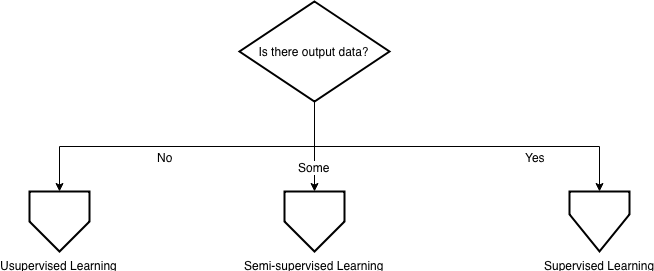
\includegraphics[width=\textwidth]{main-decision}
  \caption{Deciding the class of machine learning to use}
  \label{main-decision}
\end{figure}

If the dataset has no output data, it is classed as an Unsupervised Learning problem. Within Unsupervised Learning, if there are lots of features in the dataset, suggest using a Self-Organizing Map to analyze. Otherwise judge whether the dataset have structure or not. If they have structure, suggest K-means Clustering to analyze, otherwise suggest using Principal Component Analysis. This deicion is modelled in figure \ref{unsupervised-decision}.

\begin{figure}[h!]
  \centering
  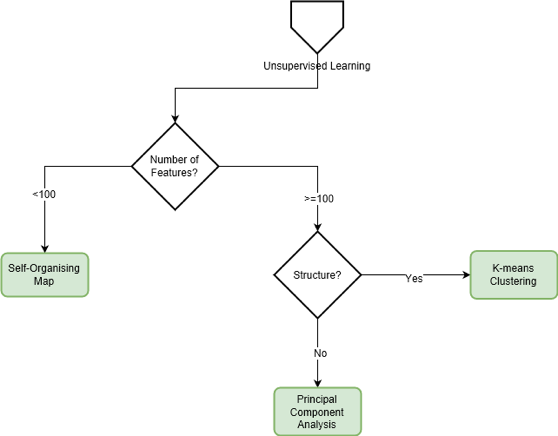
\includegraphics[width=\textwidth]{unsupervised-decision}
  \caption{Deciding which unsupervised learning technique to suggest}
  \label{unsupervised-decision}
\end{figure}

If the dataset is completely labelled with output data, divide it into Supervised Learning. If the outputs are categories divide the dataset to Classification. Else if the outputs are continuous values, divide the dataset to Regression.

If the dataset is best modelled by classification, determine how many categories the dataset contains. If dataset contains 3 or more categories, determine if the dataset is simple or not. For small complex datasets, suggest Multiclass Neural Network or Random Forest Regression. For simple large dataset, suggest using Multiclass Logistic Regression to analyze. If the dataset only contains less than 3 categories, determine whether the relation in the dataset is simple. If the dataset has simple relations, suggest Logistic Regression. Otherwise determine how many features in the dataset. If the dataset has less than 100 features, suggest Neural Network, otherwise suggest Naïve Bayesian Classifier or Support Vector Machine. If, after modelling the data using a Naïve Bayesian Classifier or Support Vector Machine, the output is worse than a guess, suggest Anti-learning.

If the dataset is composed of values (regression), also determine the dataset simple or not, if it is a simple large dataset, suggest Linear Regression. Else if a complex small dataset, suggest Random Forest Regression and Sum Regression. Figure \ref{supervised-decision} vizualises this set of decisions.

\begin{figure}[h!]
  \centering
  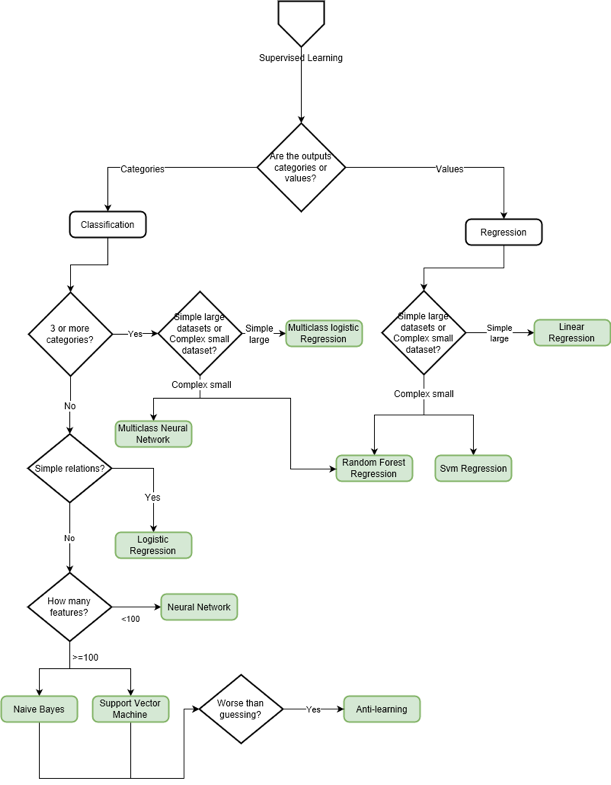
\includegraphics[width=\textwidth]{supervised-decision}
  \caption{Deciding which supervised learning technique to suggest}
  \label{supervised-decision}
\end{figure} \pagebreak

\section{Key Implementation Decisions}
\subsection{Programming Languages}
When deciding which languages would be most suitable for the project, a few aspects that were considered were functionality, familiarity  and convenience. Functionality was the main concern, given that the system is a web-based project. Therefore, the group needed to choose a language that could interface easily with a web application. Familiarity made this decision more difficult, as only one group member was familiar with JavaScript, which is the main language used on the web. As such, the group had to pick a range of languages that accomodated both the functionality needed as well as the experience level of the group members. Convenience therefore became an issue, as all group members had to ensure that code in one language could easily interface with code from another language.

Apart from HTML and CSS, both of which are essential to any web application, a few languages discussed are listed below.
\begin{enumerate}
  \item JavaScript
  JavaScript is a web scripting language. JavaScript enables interactive web pages and thus is an essential part of web applications. It is a dynamic\cite{js_datatypes} weakly typed language. Its primary purpose is to provide interactivity and have programatic control over elements on a web-page \cite{jsWhatIsJavascript}. As a simple web-based project, most functionality needed at this stage can be implement by JavaScript. JavaScript also has an extensive collection of libraries, as well as a server-side runtime environment (Node.js \cite{nodejs}), which makes it suitable to use in the back-end of a web application. As discussed in section \ref{dbdesign}, a NoSQL MongoDB database was chosen, and Node.js contains a library (Mongoose \cite{mongoose}) which makes implementing the database easy with a Node.js framework.

  \item PHP
  PHP is a scripting language tailored for the web \cite{php}. PHP code can be integrated into Java, C and Perl and can be embedded into HTML code. It is weakly typed\cite{php_datatypes} and has a high developing efficiency to complete an activity web page. It is easy to learn, the source code can be found easily on webpages. It also can connect MongoDB. It could be used to develop server-side functionality of the project.

  \item Java
  Java is the language the group is most familiar with. There exist good Integrated Development Environments (IDEs) such as Eclipse and IntelliJ which we have all used before. It has a security structure and easy to debug. But the code would be more verbose than other languages and it is more difficult to make connection with HTML webpage. In other words, Java is suitable for some big projects that need precise design. Java code could be implemented on webpages with Java Server Pages \cite{jsp}, but this would add a lot of uneccessary overhead.

  \item Python
  Python is a language with simple structure. It is easy to master and can implement functions in fewer lines code. The shortcoming is that it is unfamiliar to the group, and so choosing it might cause unpredictable problems such as environment building which lead to the work goes slowly. Python code can be implemented on webpages via the Common Gateway Interface (CGI) \cite{python_web}.
\end{enumerate}

Due to both convenience and functionality, as described above, the group decided the main language used to implement the system would be JavaScript. It should be noted that due to limitation in its ability to perform machine learning algorithms on large datasets (a task that languages such as Python and R are very well established in), the group may have to incorporate other languages. However, JavaScript proves both convenient and capable enough for the first iterations of the system. Due to its low learning curve and past experience in the group, it will not be too difficult for everyone who needs to use it to learn enough to produce a capable system.

\subsection{Design Pattern}
As outlined in section \ref{work_division}, the group has divided the workload into three parts: Machine Learning, Database Implementation and Front End Development. These three elements of the system match the description of the \textit{Model-View-Controller} (MVC) design pattern \cite{google_mvc}. This allows for better code organisation and maintainability \cite{google_mvc} by seperating responsibilities within the codebase. The three key components of the MVC design pattern are outlined below:
\begin{itemize}
  \item Model
  This is where the data of the system is stored. The Model has no access to the View or the Controller, and is only responsible for storing the data. This is essentialy the Database part of the project.
  \item View
  The View is what is presented to the user. This is how the user inteacts with the system: the Front-End. Although the user interacts with the View, the View has no responsibilities apart from to display the data in the Model.
  \item Controller
  The Controller acts as the bridge between the Model and the View; it updates the View when changes happen to the Model, and updates the Model when the user interacts with the View. This is the Machine Learning section of the group's work division. The controller is responsible for all logic in the system.
\end{itemize}

As well as the productivity improvements outlined in section \ref{work_division}, using this design pattern increases the maintainability of the code base, as it is easier to identify where bugs occur if code with different responsibilities is seperated out. It also helps minimise the number of dependencies within the code, which makes the code more testable.

\subsection{Database Design\label{dbdesign}}
\subsubsection{NoSQL vs SQL}
Heterogenous big data benefits from NoSQL for a few reasons. Firstly, there is no predefined schema that the data has to conform to, which is useful for our application as it will have to save data from a multitude of different data sources in the same data store. It is not possible to index all the data efficiently beforehand, and therefore a large schema that all datasets will conform to cannot be defined. Even if this was easily possible, a large schema would waste a lot of space, as most datasets would only use a small subset of the schema. This would also make searching the database very inefficient, as it would be resource inefficient to have to search through potentially hundreds of unused fields.

Removing schemas also makes the database faster to query \cite{sqlvsnosql}. Because each dataset is stored in one document rather than spread across multiple tables, the program knows exactly where to look for the data set rather than having to search through multiple tables. This helps when having to search through a lot of datasets to find the data set of interest.

\subsubsection{Lack of Relations Between Datasets}
The data sets that our program will use contain almost no relations. As such, using a relational database would waste a lot of the functionality associated with relations, and cause a lot of uneccessary overhead. Instead, a non-relational database will just store data sets independently of each other. Querying the database will simply involve returning a JSON object, with no links to other data sets.

\subsection{Accepted File Types in the System}

When studying Weka, the team found that there are many file types that machine learning tools could use, for instance Arff data files, CSV data files, XRFF data files, amongst others. After some research into the UCI Machine Learning Repository \cite{uci}, the team decided to use CSV data files to store datasets into the database and to be used by the machine learning tools. This is because CSV files make it convenient for the team to transform the .data files and .name files found on the UCI repository into a single file. CSV files are also easy to store in the NoSQL database. Knowing the format of the data is useful for data pre-processing and analysing.

\section{Problems Encountered}

\subsection{Testing}

\section{Time Planning and Project Management}
At the very start of the project, time planning was discussed but was not followed or enforced as much as it should have been. As such, a Gantt Chart was devised and is shown in figure \ref{ganttchart}. This Gantt chart has helped us stick to deadlines and structure our work.

\begin{figure}\label{ganttchart}
  
\end{figure}

Alongside the Gantt chart, the team has a Kanban board which is hosted on Trello.com \cite{trello}. Scrum was discussed as an alternative approach, but Kanban was chosen for some reasons outlined below:

\begin{itemize}
% \item For a little team like ours which has only 5 members, agile provides a more suitable framework for software development.
\item Teams using Kanban can cope with mutable requirements flexibly. Teamwork will continue with changing project environment.
\item Formal and informal meetings can be held as frequently as needed and agile working process can be pushed favorably by team communication.
\item Due to the main process of the project having been decided, Kanban is a good system as it allows us to vizualise every stage of work and everyone’s processing.
\item For a team with less development experience, it is difficult to deliver an executable program in a short time. Scrum would be difficult to practice because of its demand on techniques and experience.
\item Scrum need to stipulate working time for every iteration, which is difficult for teams with less development experience. Kanban only displays stage missions but not time limits.
\item Scrum needs to declare a Product Owner, Scrum manager and Team which might cause confusion in an inexperienced team. Kanban can make team members focus on their work and research.
\end{itemize}

After agreeing that Kanban would be more suitable to our team's needs, a Kanban board was created on Trello. Trello was chosen as it makes collaboration a lot easier. Being a web based tool, it made it easy for us to manage our workflow from all of our devices, as well as accomodating remote work and management. It also allows team collaboration as it allows people to join the Trello board, which was an essential feature the team needed in order to be able to manage its work collaboratively.

\subsection{Division of Work\label{work_division}}
Rather than everyone playing a role in every aspect of the project, it was decided it would be easier to divide the work into three distinct subgroups. The project was divided into three main sections: \textit{Front-End Development}, \textit{Machine Learning} and \textit{Data Pre-processing and Database Development}. It was decided that Hao and Xinyang would be responsible for Front-End Development, Boyan and Xinjie for Machine Learning and Marios for the Data Processing and Database. The division was made based on both past experience with technologies needed for that area, as well as personal preference. As such, there was no conflict in deciding who would be responsible for what area.

Dividing the project in this fashion allowed the team to be able to divide workload more efficiently, as any task could be categorised into one of the three areas of the project and assign the task to the correct person(s).

Following this division of labour, it was decided that the Kanban board would be better organised if there was a list for each section. Therefore, three lists ("To Do", "Doing" and "Done") were created for each are of the project, as well as one set of lists for "Other" tasks that had to be done (for example, adding a section to the report, drawing diagrams). This project management workflow kept everything atomic, where everyone was only responsible for a small subset of tasks. It also kept people focused, as everyone could find the correct list for their section and pick up "To Do" tasks that correspond to their section of the project.

\pagebreak
\printbibliography

\end{document}